% Remaining controller configuration and workflow figures, integrated in Appendix C.

\begin{figure}[!htbp]
  \begin{adjustwidth}{-\extralength}{0cm}
  \centering
  \includegraphics[width=\fulllength,height=0.88\textheight,keepaspectratio]{figures/04_fuzzy_rules_panel_5labels.png}
  \end{adjustwidth}
  \caption{Rule-base consequents R1--R8 at $n=5$. Rows denote diversity labels and columns denote progress labels.}
  \label{fig:rule_panel_5}
\end{figure}

\begin{figure}[p]
  \begin{adjustwidth}{-\extralength}{0cm}
  \centering
  \includegraphics[width=\fulllength,height=0.88\textheight,keepaspectratio]{figures/04_fuzzy_rules_panel_7labels.png}
  \end{adjustwidth}
  \caption{Rule-base consequents R1--R8 at $n=7$. Rows denote diversity labels and columns denote progress labels.}
  \label{fig:rule_panel_7}
\end{figure}

\begin{figure}[p]
  \begin{adjustwidth}{-\extralength}{0cm}
  \centering
  \includegraphics[width=\fulllength,height=0.88\textheight,keepaspectratio]{figures/04_fuzzy_rules_panel_9labels.png}
  \end{adjustwidth}
  \caption{Rule-base consequents R1--R8 at $n=9$. Rows denote diversity labels and columns denote progress labels.}
  \label{fig:rule_panel_9}
\end{figure}

\begin{figure}[p]
  \centering
  \includegraphics[width=0.92\textwidth,height=0.82\textheight,keepaspectratio]{figures/11_3d_surface_panel_3labels_I1.png}
  \caption{Effective Mamdani inertia-weight surfaces for R1--R8 at $n=3$, over diversity and progress; $w\in[0.1,0.9]$.}
  \label{fig:surface_panel_3}
\end{figure}

\begin{figure}[p]
  \centering
  \includegraphics[width=0.92\textwidth,height=0.82\textheight,keepaspectratio]{figures/11_3d_surface_panel_7labels_I1.png}
  \caption{Effective Mamdani inertia-weight surfaces for R1--R8 at $n=7$, over diversity and progress; $w\in[0.1,0.9]$.}
  \label{fig:surface_panel_7}
\end{figure}

\begin{figure}[p]
  \centering
  \includegraphics[width=0.92\textwidth,height=0.82\textheight,keepaspectratio]{figures/11_3d_surface_panel_9labels_I1.png}
  \caption{Effective Mamdani inertia-weight surfaces for R1--R8 at $n=9$, over diversity and progress; $w\in[0.1,0.9]$.}
  \label{fig:surface_panel_9}
\end{figure}

\usetikzlibrary{positioning,fit,shapes.geometric}
\begin{figure}[p]
  \begin{adjustwidth}{-\extralength}{0cm}
  \centering
  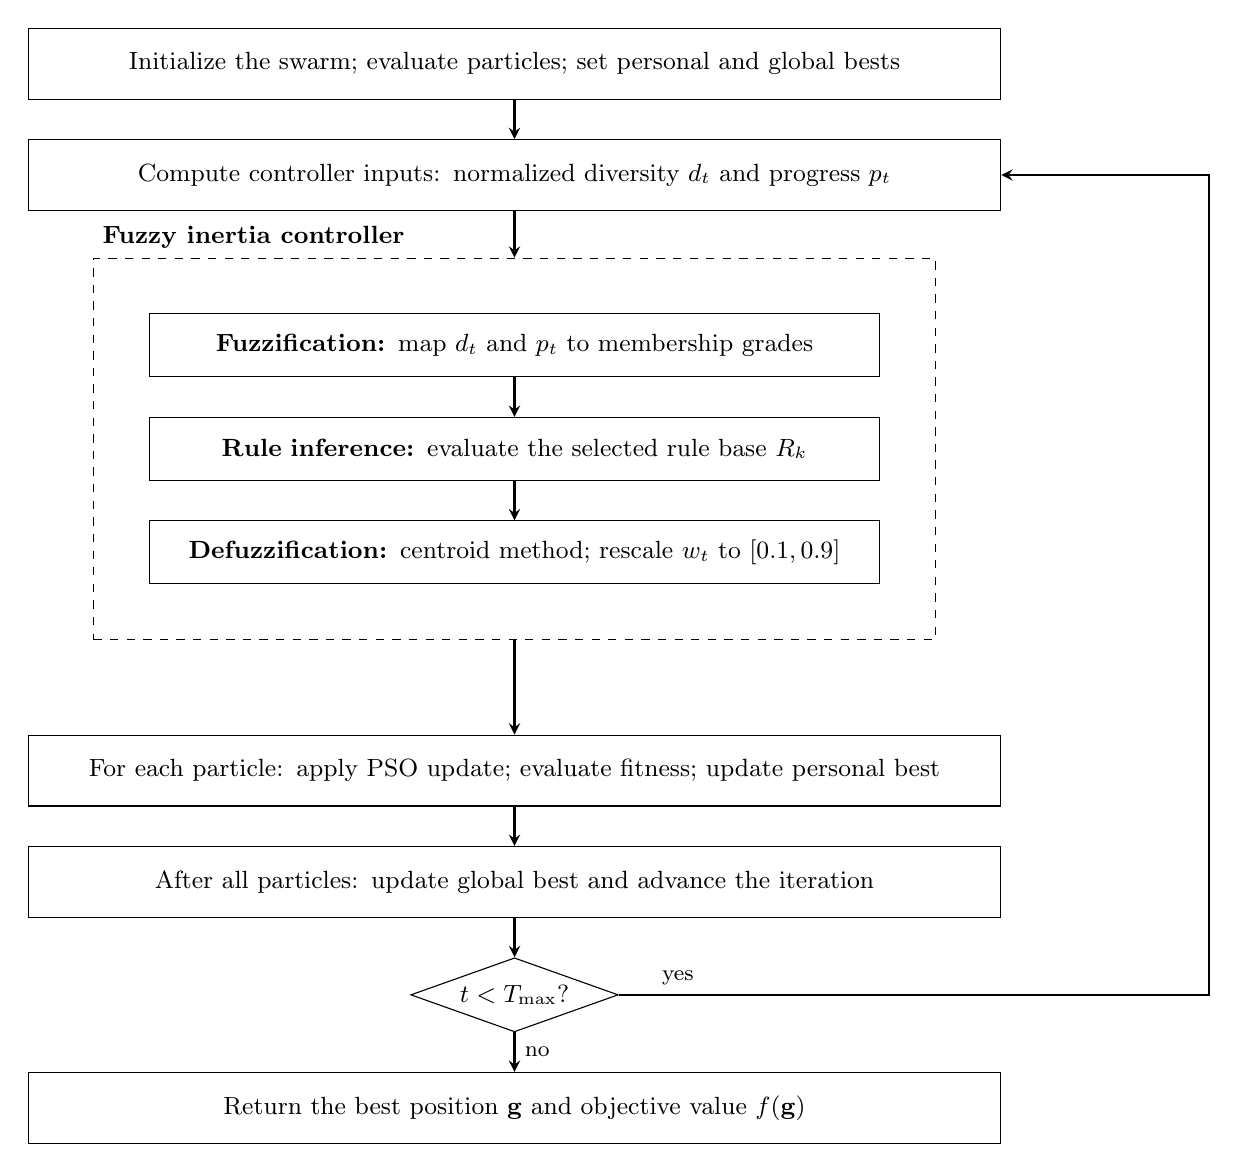
\begin{tikzpicture}[
    process/.style={draw=black,fill=white,rectangle,align=center,text width=12cm,minimum height=9mm,inner sep=5pt,font=\small},
    controller/.style={draw=black,fill=white,rectangle,align=center,text width=9cm,minimum height=8mm,inner sep=4pt,font=\small},
    decision/.style={draw=black,fill=white,diamond,aspect=2.8,align=center,inner sep=2pt,font=\small},
    flow/.style={->,>=stealth,thick,draw=black},
    node distance=5mm]
    \node[process] (initialize) {Initialize the swarm; evaluate particles; set personal and global bests};
    \node[process,below=of initialize] (state) {Compute controller inputs: normalized diversity $d_t$ and progress $p_t$};
    \node[controller,below=13mm of state] (fuzzify) {\textbf{Fuzzification:} map $d_t$ and $p_t$ to membership grades};
    \node[controller,below=of fuzzify] (infer) {\textbf{Rule inference:} evaluate the selected rule base $R_k$};
    \node[controller,below=of infer] (defuzzify) {\textbf{Defuzzification:} centroid method; rescale $w_t$ to $[0.1,0.9]$};
    \node[draw=black,dashed,rectangle,fit=(fuzzify)(infer)(defuzzify),inner sep=7mm,
      label={[anchor=south west,font=\small]north west:\textbf{Fuzzy inertia controller}}] (fis) {};
    \node[process,below=12mm of fis] (particle) {For each particle: apply PSO update; evaluate fitness; update personal best};
    \node[process,below=of particle] (swarm) {After all particles: update global best and advance the iteration};
    \node[decision,below=of swarm] (continue) {$t<T_{\max}$?};
    \node[process,below=of continue] (result) {Return the best position $\mathbf{g}$ and objective value $f(\mathbf{g})$};
    \draw[flow] (initialize) -- (state);
    \draw[flow] (state.south) -- (fis.north);
    \draw[flow] (fuzzify) -- (infer);
    \draw[flow] (infer) -- (defuzzify);
    \draw[flow] (fis.south) -- (particle.north);
    \draw[flow] (particle) -- (swarm);
    \draw[flow] (swarm) -- (continue);
    \draw[flow] (continue) -- node[right,font=\footnotesize]{no} (result);
    \draw[flow] (continue.east) -- node[above,font=\footnotesize]{yes} ++(15mm,0) -- ++(60mm,0) |- (state.east);
  \end{tikzpicture}
  \end{adjustwidth}
  \caption{PSO--FCS workflow: the common two-input fuzzy controller returns one inertia weight shared by all particles.}
  \label{fig:pso_fcs_loop}
\end{figure}